\chapter{Proceso de software ejecutado}\label{Proceso de software ejecutado}
%Función que crea el título de capítulo y al cual se le da el nombre deseado a través de su parámetro obligatorio. Al no tener la función el “*” se escribirá también en el título del documento las palabras “Capítulo 1: …”. Además se indica, mediante la función “\label”, la correspondiente etiqueta que lleva asociada. La etiqueta sirve para que en caso de que luego se quiera hacer referencia al capítulo se haga llamando etiqueta tal que se escribiría “La información correspondiente a dicho tema se encuentra en el capítulo \ref{Int}.”

\thispagestyle{fancy}
%Función que determina que durante este capítulo se aplique el estilo Fancy.

\fancyhead[LE]{\thechapter.Proceso de software ejecutado} 
%Función que se utiliza para indicar que en las páginas impares, aparezca en el encabezado en la parte izquierda, el número del capítulo con su correspondiente nombre.

En este capitulo, se va a explorar los requisitos del proyecto, el diseño seguido para cumplirlo, el desarrollo para poner en practica la idea y por ultimo la validación para comprobar su funcionamiento.

\section{Análisis}
Para poder resolver los problemas de identidad del mundo, hay que crear una lista de requisitos. Después de realizar nuestro desarrollo, se volverá a visitar la lista para concluir si nuestro desarrollo ha sido satisfactorio.

\subsection{Requisitos (funcionales y no funcionales)}
Antes de comenzar a desarrollar la solución, hay que analizar las posibilidades y elegir las librerías correctas.

\definecolor{Gray}{gray}{0.9}

\begin{center}
    \begin{table}[h!]
        \begin{tabular}{|p{0.1\linewidth} | p{0.8\linewidth}|}
            \hline
            \rowcolor{Gray} 
            \textbf{O1} & \textbf{Diseño de un sistema de SSI distribuido.} \\
            \hline
            RF1         & La plataforma debe contar con una pagina web estática. \\
            \hline
            RF2         & La plataforma debe poder enviar datos en un medio distribuido. \\
            \hline
            RF3         & La plataforma debe comunicarse con una red blockchain. \\
            \hline
            RF4         & La plataforma debe poder identificar usuarios en un mundo medio distribuido. \\
            \hline
            RF5         & La plataforma debe procesar peticiones de los usuarios en un medio distribuido. \\
            \hline
            RNF1        & La plataforma debe ser \textit{open source}. \\
            \hline
            RNF2        & La plataforma debe usar librerías \textit{open source}. \\
            \hline
        \end{tabular}
    \end{table}
\end{center}
\textbf{La plataforma debe contar con una pagina web estática.}\\
Para poder desplegar nuestra aplicación web en IPFS \cite{web:ipfs}, necesitamos que nuestra página sea estática. Esto significa que no podemos generar nuestro HTML en un servidor.
\begin{center}
    \begin{table}[h!]
        \begin{tabular}{|p{0.1\linewidth} | p{0.8\linewidth}|}
            \hline
            \rowcolor{Gray} 
            \textbf{O1-RF1} & \textbf{La plataforma debe contar con una pagina web estática.} \\
            \hline
            S111            & Empaquetado de \textit{assets}. \\
            \hline
            S112            & Optimización de código. \\
            \hline
            S113            & \textit{Code splitting.} \\
            \hline
        \end{tabular}
    \end{table}
\end{center}
\begin{itemize}
    \item \textbf{S111}: La herramienta, debe tener una opción para poder empaquetar HTML, JS y CSS en un solo fichero JS.
    \item \textbf{S112}: La herramienta, debe optimizar nuestra aplicación para que tenga un mejor rendimiento.
    \item \textbf{S113}: La herramienta, debe poder dividir nuestro payload en diferentes ficheros para no tener que enviar un archivo excesivamente grande.
\end{itemize}
\textbf{La plataforma debe poder enviar datos en un medio distribuido.}\\
Ya que se quiere implementar un sistema de identidades distribuidas, necesitaremos un canal por el que poder comunicar a todos los usuarios.
\begin{center}
    \begin{table}[h!]
        \begin{tabular}{|p{0.1\linewidth} | p{0.8\linewidth}|}
            \hline
            \rowcolor{Gray} 
            \textbf{O1-RF2} & \textbf{La plataforma debe poder enviar datos en un medio distribuido.} \\
            \hline
            S121            & Capacidad de mutar datos. \\
            \hline
            S112            & Seguro. \\
            \hline
        \end{tabular}
    \end{table}
\end{center}
\begin{itemize}
    \item \textbf{S121}: La herramienta, tiene que ser capaz de proporcionar las herramientas necesarias de mutar datos. Este paso es esencial si se necesita implementar una base de datos.
    \item \textbf{S122}: La herramienta, tiene que poder asegurarnos que el transporte de los datos es seguro entre nodos para evitar la suplantación de identidad.
\end{itemize}
\textbf{La plataforma debe comunicarse con una red blockchain.}\\
Para poder verificar que el usuario es quien dice ser, necesitamos un medio que nos garantice la trazabilidad de las identidades sin revelar los datos personales de las mismas.
\begin{center}
    \begin{table}[h!]
        \begin{tabular}{|p{0.1\linewidth} | p{0.8\linewidth}|}
            \hline
            \rowcolor{Gray} 
            \textbf{O1-RF3} & \textbf{La plataforma debe comunicarse con una red blockchain.} \\
            \hline
            S131            & Exponer un método de comunicación desde la interfaz. \\
            \hline
            S132            & Compatible con librerías de escucha a contratos. \\
            \hline
        \end{tabular}
    \end{table}
\end{center}
\begin{itemize}
    \item \textbf{S131}: La herramienta, tiene que exponer un puerto de comunicación desde el que se pueda enviar y recibir información.
    \item \textbf{S132}: La herramienta, tiene que ser compatible con librerías de escucha a contratos para poder responder a eventos que ocurran.
\end{itemize}
\textbf{La plataforma debe poder identificar usuarios en un mundo medio distribuido.}\\
A fecha de publicación de este trabajo, la web todavía no dispone de un estándar para las identidades distribuidas. Aún así, existe una propuesta en camino de ser aceptada \cite{web:did-spec}.
\begin{center}
    \begin{table}[h!]
        \begin{tabular}{|p{0.1\linewidth} | p{0.8\linewidth}|}
            \hline
            \rowcolor{Gray} 
            \textbf{O1-RF4} & \textbf{La plataforma debe poder identificar usuarios en un mundo medio distribuido.} \\
            \hline
            S141            & Decodificar DID. \\
            \hline
            S142            & Codificar DID. \\
            \hline
        \end{tabular}
    \end{table}
\end{center}
\begin{itemize}
    \item \textbf{S141}: La herramienta, debe ser capaz de decodificar los DID y obtener la información necesaria.
    \item \textbf{S142}: La herramienta, debe ser capaz de codificar el DID del usuario accediendo a su cartera.
\end{itemize}
\textbf{La plataforma debe procesar peticiones de los usuarios en un medio distribuido.}\\
Al no disponer de un backend, tenemos que diseñar una alternativa para conseguir la misma funcionalidad utilizando el mundo distribuido. En vez de usar un patrón de diseño REST, se va a utilizar gRCP. Esto se debe a que nuestro backend, no tiene datos los cuales puede devolver. Solo podemos ejecutar funciones.
\begin{center}
    \begin{table}[h!]
        \begin{tabular}{|p{0.1\linewidth} | p{0.8\linewidth}|}
            \hline
            \rowcolor{Gray}
            \textbf{O1-RF5} & \textbf{La plataforma debe procesar peticiones de los usuarios en un medio distribuido.} \\
            \hline
            S151            & Exponer funciones para ser llamadas desde los usuarios. \\
            \hline
        \end{tabular}
    \end{table}
\end{center}
\begin{itemize}
    \item \textbf{S151}: Siguiendo un patrón gRCP, se expondrán funciones con las se podrán llamar desde la aplicación.
\end{itemize}
\textbf{La plataforma debe ser \textit{open source}.}\\
Para asegurar un desarrollo ético de este proyecto, se desarrollará bajo una licencia open source. Más adelante se explicarán las implicaciones éticas de este proyecto.
\begin{center}
    \begin{table}[h!]
        \begin{tabular}{|p{0.15\linewidth} | p{0.75\linewidth}|}
            \hline
            \rowcolor{Gray} 
            \textbf{O1-RNF1} & \textbf{La plataforma debe ser \textit{open source}.} \\
            \hline
            S11N1            & Licencia \textit{open source}. \\
            \hline
        \end{tabular}
    \end{table}
\end{center}
\begin{itemize}
    \item \textbf{S11N1}: Para asegurar que el proyecto y los próximos que avancen lo creado en este, se usará una licencia que lo pueda asegurar. \textbf{GNU General Public License v3.0}.
    \begin{table}[h!]
        \centering
        \begin{tabular}{|c|c|c|}
            \hline
            Permissions         & Limitations   & Conditions \\
            \hline
            Commercial use      & Liability     & License and copyright notice \\
            \hline
            Modification        & Warranty      & State changes \\
            \hline
            Distribution        &               & Disclose source\\
            \hline
            Patent use          &               & Same license \\
            \hline
            Private use         &               & \\
            \hline
        \end{tabular}
        \cite{web:LICENSE}
    \end{table}
\end{itemize}
\textbf{La plataforma debe usar librerías open source.}
Este proyecto, al ser open source, utilizará multiples librerías, todas ellas de código abierto. De esa manera, cualquier fragmento de código puede ser verificado.
\begin{center}
    \begin{table}[h!]
        \begin{tabular}{|p{0.15\linewidth} | p{0.75\linewidth}|}
            \hline
            \rowcolor{Gray} 
            \textbf{O1-RNF2} & \textbf{La plataforma debe usar librerías \textit{open source}.} \\
            \hline
            S11N2            & Licencia \textit{open source}. \\
            \hline
        \end{tabular}
    \end{table}
\end{center}
\begin{itemize}
    \item \textbf{S12N1}: Las librerías usadas deberán usar licencias de código abierto.
\end{itemize}
\noindent\rule{\textwidth}{0.4pt}
\newpage
\begin{center}
    \begin{table}[h!]
        \begin{tabular}{|p{0.1\linewidth} | p{0.8\linewidth}|}
            \hline
            \rowcolor{Gray} 
            \textbf{O2} & \textbf{Desarrollo de un sistema de SSI distribuido.} \\
            \hline
            RF1     & La plataforma debe ejecutar un nodo IPFS \cite{web:ipfs}. \\
            \hline
            RF2     & La plataforma debe contar con las APIs necesarias para comunicarse con la cartera del usuario.\\
            \hline
            RF3     & La plataforma debe ejecutar una base de datos orbit db. \\
            \hline
        \end{tabular}
    \end{table}
\end{center}
\textbf{La plataforma debe ejecutar un nodo IPFS \cite{web:ipfs}.}\\
Como la herramienta elegida ha sido IPFS \cite{web:ipfs}, se necesitará asegurar su correcto funcionamiento.
\begin{center}
    \begin{table}[h!]
        \begin{tabular}{|p{0.15\linewidth} | p{0.75\linewidth}|}
            \hline
            \rowcolor{Gray} 
            \textbf{O2-RF1} & \textbf{La plataforma debe ejecutar un nodo IPFS \cite{web:ipfs}.} \\
            \hline
            S211     & Configuración correcta con servidores star. \\
            \hline
            S212     & Configuración correcta de orbit db. \\
            \hline
            S213     & Generar métodos para descargar datos y desencriptarlos. \\
            \hline
            S214     & Generar métodos para subir datos y encriptarlos. \\
            \hline
        \end{tabular}
    \end{table}
\end{center}
\begin{itemize}
    \item \textbf{S211}: Se deberá configurar IPFS \cite{web:ipfs} correctamente para que los usuarios se puedan encontrar entre ellos.
    \item \textbf{S212}: Para que las bases de datos se puedan replicar correctamente, orbit db necesita estar configurado correctamente.
    \item \textbf{S213}: Para poder subir información a IPFS \cite{web:ipfs}, necesitaremos que esté encriptada para la seguridad del usuario.
    \item \textbf{S214}: Para descargar información de IPFS \cite{web:ipfs}, necesitaremos desencriptarlos.
\end{itemize}
\textbf{La plataforma debe contar con las APIs necesarias para comunicarse con la cartera del usuario.}\\
Para poder comunicarnos con la cartera necesitaremos utilizar el objeto \verb|window.ethereum| correctamente.
\begin{center}
    \begin{table}[h!]
        \begin{tabular}{|p{0.15\linewidth} | p{0.75\linewidth}|}
            \hline
            \rowcolor{Gray} 
            \textbf{O2-RF2} & \textbf{La plataforma debe contar con las APIs necesarias para comunicarse con la cartera del usuario.} \\
            \hline
            S221     & Métodos auxiliares para usar la funcionalidad de la cartera \\
            \hline
        \end{tabular}
    \end{table}
\end{center}
\begin{itemize}
    \item \textbf{S221}: Se crearán métodos generalistas para poder comunicarse con metamask.
\end{itemize}
\textbf{La plataforma debe ejecutar una base de datos orbit db.}\\
Para poder ejecutar una base de datos, se necesitará crear una instancia de IPFS \cite{web:ipfs}.
\begin{center}
    \begin{table}[h!]
        \begin{tabular}{|p{0.15\linewidth} | p{0.75\linewidth}|}
            \hline
            \rowcolor{Gray} 
            \textbf{O2-RF3} & \textbf{La plataforma debe contar con las APIs necesarias para comunicarse con la cartera del usuario.} \\
            \hline
            S231     & Generar claves para la comunicación. \\
            \hline
            S232     & Generar base de datos \textit{keyvalue}. \\
            \hline
            S233     & Generar métodos de escucha de eventos. \\
            \hline
            S234     & Subir DID a la base de datos. \\
            \hline
        \end{tabular}
    \end{table}
\end{center}
\begin{itemize}
    \item \textbf{S231}: Para poder iniciar la comunicación, necesitaremos generar las claves publica y privada.
    \item \textbf{S232}: Se necesitará crear una base de datos \textit{keyvalue}.
    \item \textbf{S233}: Para poder avisar al usuario de lo que ocurra, hay que poder escuchar a eventos en la red.
    \item \textbf{S234}: Para presentar al usuario ante el resto, habrá que subir nuestra identificación a la base de datos.
\end{itemize}
\section{Diseño}
En este apartado, se va a diseñar la solución para poder cumplir los requisitos del sistema.
\subsection{Arquitectura general}
\begin{figure}[h!]
    \centering
    \includegraphics[width=0.9\textwidth]{Figures/Diseño.png}
    \caption{Diseño de la aplicación. Los nodos color verde son puertos de escucha IPFS \cite{web:ipfs}. El nodo de color naranja es un puerto de escucha de MetaMask.}
\end{figure}
Este es el diseño actual de la solución. \textit{A priori}, parece imposible que pueda funcionar ya que no existe ningún tipo de \textit{backend} en el que podamos ejecutar la lógica. Toda la lógica se ejecuta utilizando \textit{smart contracts} y el resto son intercambios de datos por IPFS \cite{web:ipfs}.
La conexión de metamask con la blockchain esta fuera del área de control. Para poder interactuar con la cartera, disponemos de un canal de comunicación en el que podemos enviar mensajes.
\begin{lstlisting}
    const syncKey = await window.ethereum.request({
			method: '',
			params: [],
    });
\end{lstlisting}
Utilizando esta función, podemos enviar un \verb|method|, y unos argumentos. Los métodos, son las funcionalidades que puede hacer metamask.
Por ejemplo, para poder compartir la identidad del usuario y empezar a trabajar, tenemos que pedirle permiso. 
\begin{lstlisting}
    let encryptionPublicKey;
    ethereum
    .request({
        method: 'eth_getEncryptionPublicKey',
        params: [account], 
        // you must have access to the specified account
    })
    .then((result) => {
        encryptionPublicKey = result;
    })
    .catch((error) => {
        if (error.code === 4001) {
        // EIP-1193 userRejectedRequest error
        console.log("We can't encrypt anything without the key.");
        } else {
        console.error(error);
        }
    });
\end{lstlisting}
\cite{web:metamask_wiki}
\subsection{Modelo funcional}
A diferencia de otros frameworks clásicos que utilizan el modelo MVC (Model, View, Controller), Nextjs, aunque capaz de hacer renderizado por servidor, su función principal es generar paginas estáticas. Estas paginas, para ser renderizadas, son llamadas como una función. React, como ya se ha dicho antes, utiliza JSX, siendo capaz de añadir HTML en JS.
\begin{lstlisting}
    import Header from '../components/header';
    import HeroSection from '../components/hero';
    import Head from 'next/head';

    export default function Home() {
        return (
            <>
                <Head>
                    <title>TFG self soverign identity</title>
                    <meta name="viewport" content="initial-scale=1.0, width=device-width" />
                </Head>
                <Header />
                <HeroSection />
            </>
        );
    }
\end{lstlisting}
Para poder renderizar la pagina inicial (index), necesitamos ejecutar la función Home, que tiene un un return, que devuelve HTML.
Cuando un usuario solicita nuestra pagina, se le devuelve el HTML ya generado con el archivo JS que ha generado ese HTML en el servidor a la hora de construcción. El navegador, ejecuta ese archivo de JS hidratando la pagina y añadiendo toda la funcionalidad.
\subsection{Escucha de eventos}
\begin{figure}[h!]
    \centering
    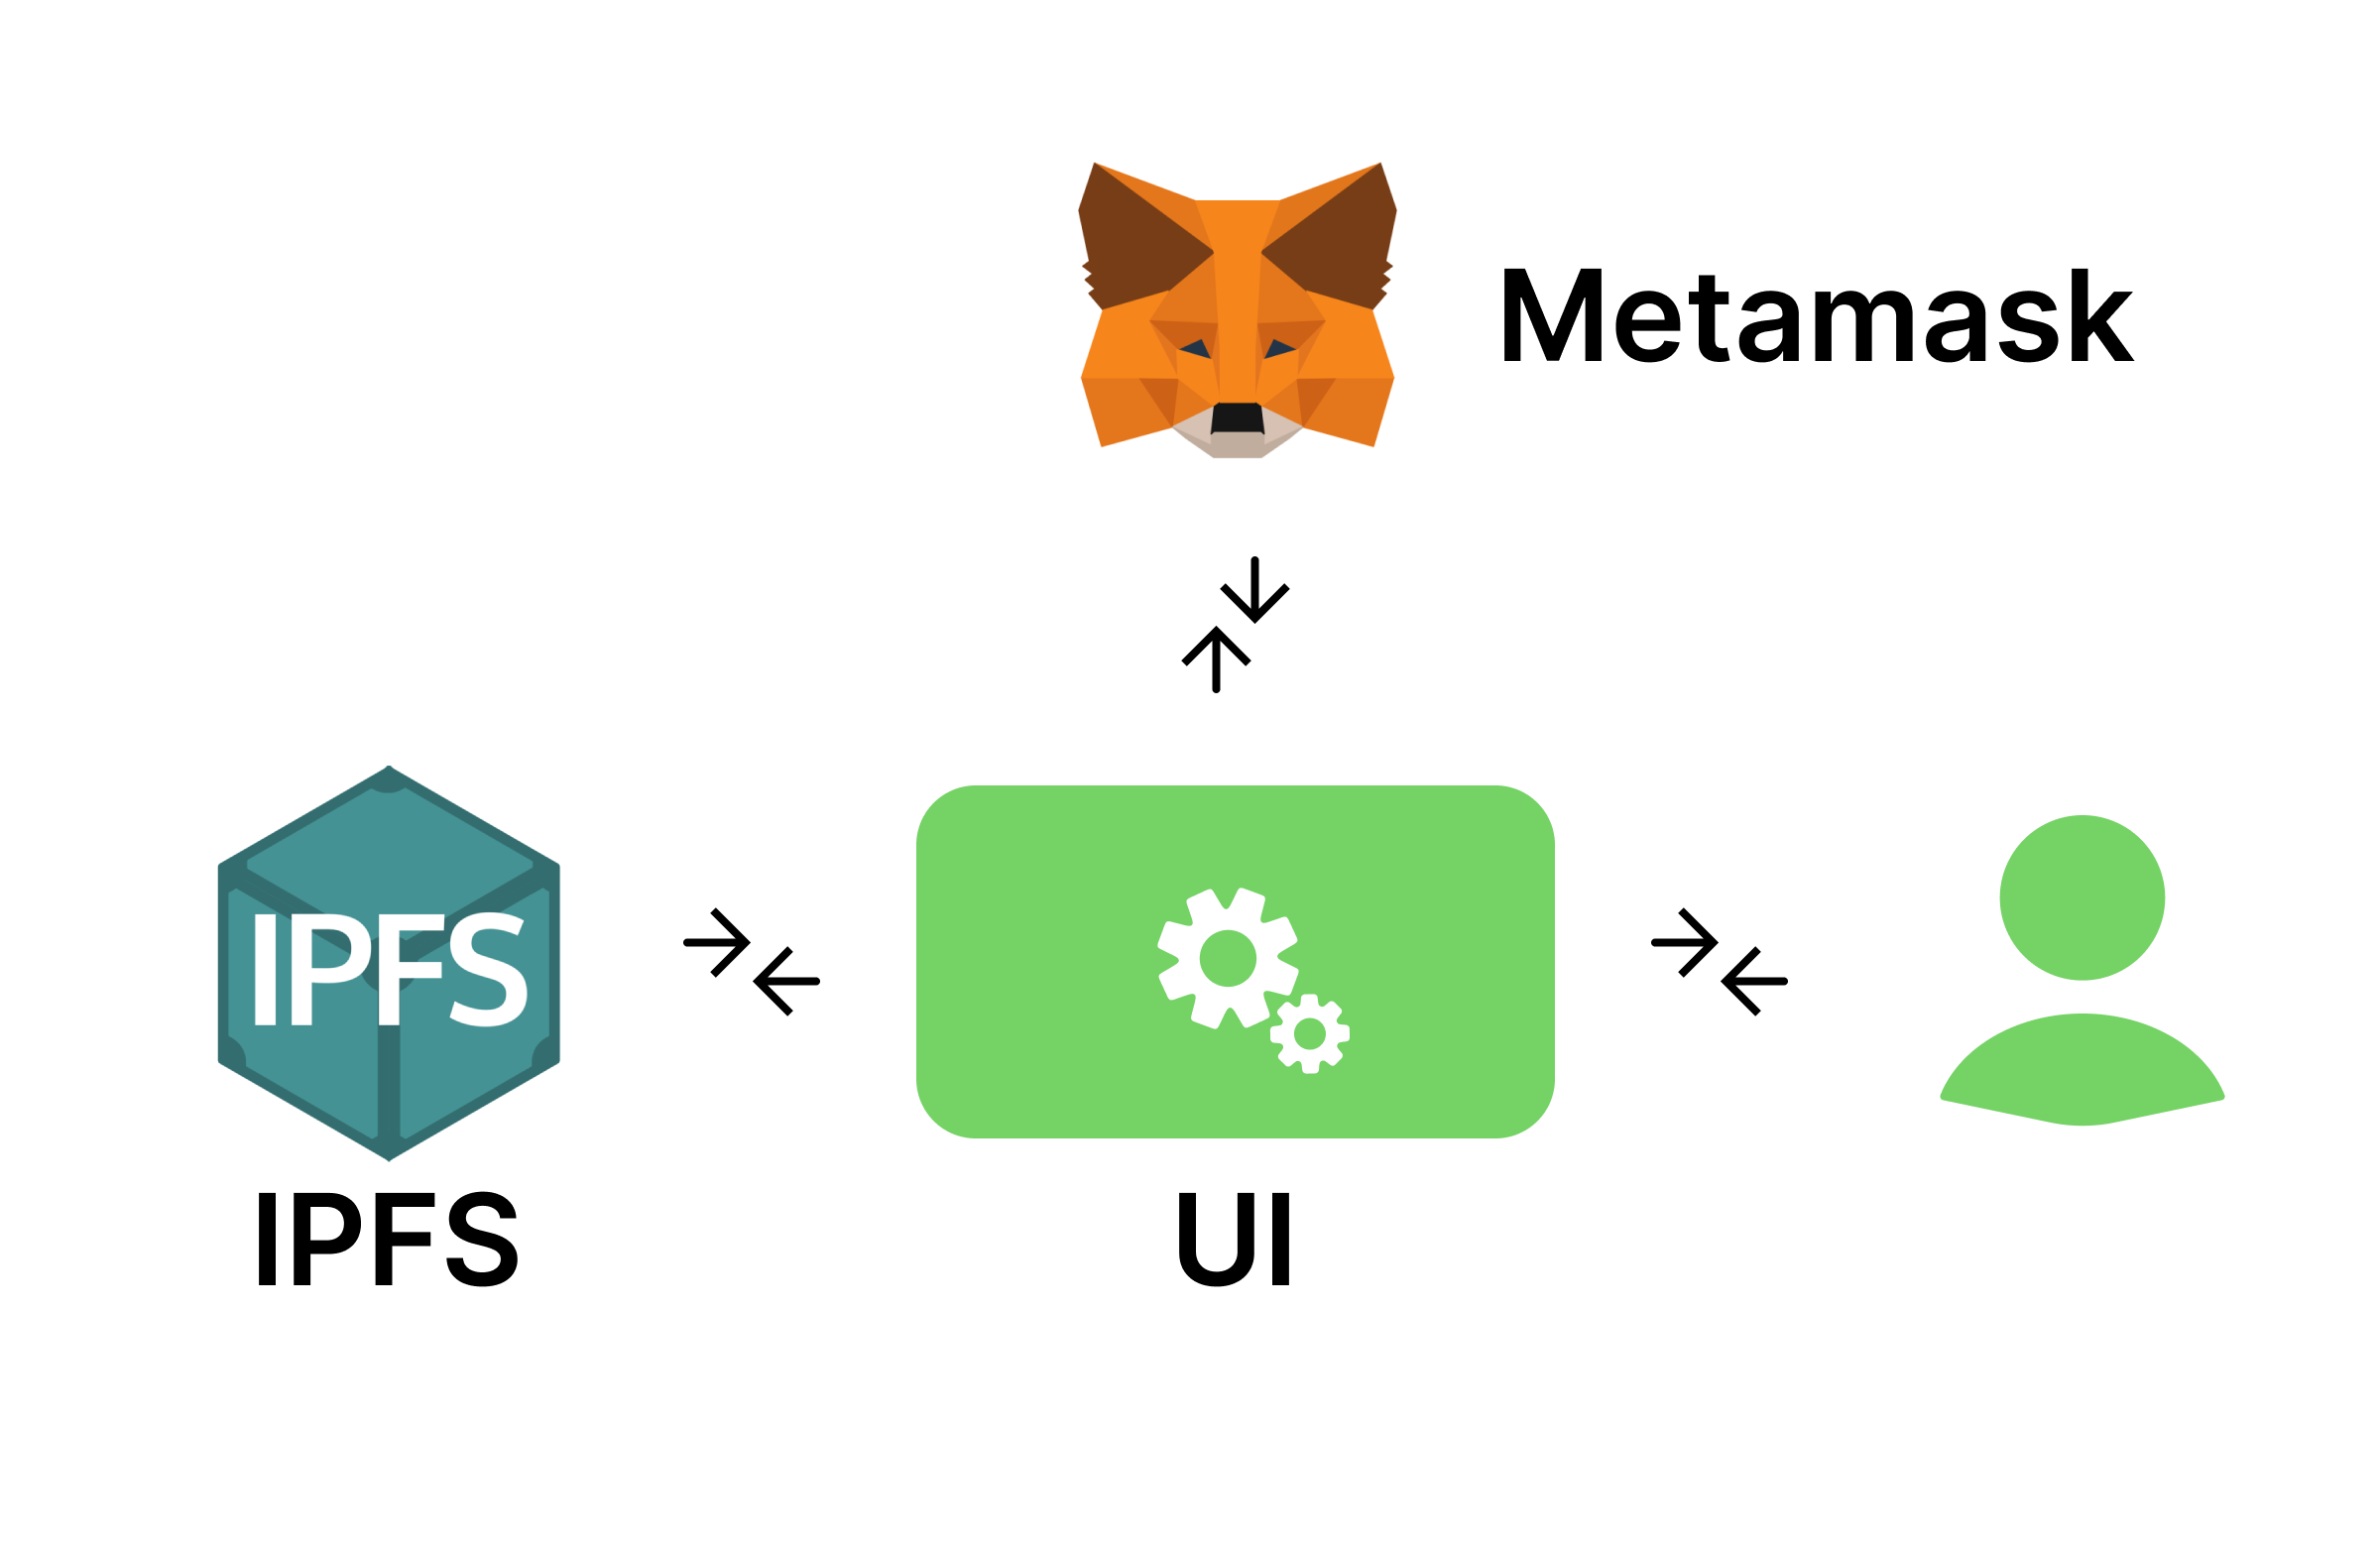
\includegraphics[width=0.9\textwidth]{Figures/Reactividad.png}
    \caption{Diagrama que muestra como la UI puede reaccionar a eventos que ocurren en la red para mostrar los cambios al ususario.}
\end{figure}
Este proyecto, una vez hidratado, es capaz de escuchar a eventos en la red. Gracias a esto, la UI es capaz de reaccionar y cambiar adecuadamente. Todo esto ocurriendo a tiempo real. Así mismo, también puede reaccionar a las acciones del usuario y reaccionar adecuadamente.
\subsection{Rutas}
Las rutas en nextjs, no son programáticas, sino contextuales. Las rutas se declaran creando archivos \verb|.js| en la carpeta pages.
\begin{lstlisting}
> tree
.
|-- _app.js
|-- index.js
|-- login.js
|-- upload.js

0 directories, 4 files
\end{lstlisting}
Este árbol, nos dice que hay tres rutas más un fichero con funcionalidad especial.
\begin{itemize}
    \item \verb|index|
    \item \verb|login|
    \item \verb|upload|
\end{itemize}
El archivo \verb|_app|, es un archivo que \textit{configura} al resto de las rutas.
Como el método de \verb|index| se llama \verb|Home|, el HTML resultante quedaría así.
\begin{lstlisting}
    <App>
        <Home/>
    </App>
\end{lstlisting}
En el método \verb|App|, podemos introducir lógica que queremos que se ejecute en cada página, incluyendo también el HTML que queremos en cada una. En este lugar, podemos establecer la lógica necesaria para comunicarnos con la cartera del usuario y una manera para poder compartir estado global a lo largo de toda la aplicación.
De este modo, al tratarse de una SPA \cite{web:spa} (Single page application), podemos mantener esa conexión sin y guardar por ejemplo la dirección del usuario o la conexión IPFS \cite{web:ipfs}.
\section{Desarrollo}
En esta sección, se va a exponer el desarrollo del proyecto siguiendo las guías establecidas en la sección de diseño.
\subsection{Entorno de desarrollo}
El entorno elegido para el desarrollo, es un ordenado fijo con un sistema operativo UNIX-like \cite{web:unix-like}. Con la ultima version de node instalada. Este sistema operativo ha sido escogido, por varios motivos. Al ser un sistema operativo centrado en la terminal, la experiencia de desarrollo, es muy superior a la que windows puede ofrecer. Así mismo, al ser un sistema operativo de código abierto, concuerda con la filosofía de este proyecto.
Así mismo, el navegador principal en el que se han realizado todas las pruebas han sido en el navegador Firefox. El cual también es código abierto.
Este sistema operativo, en especifico, Arch Linux \cite{web:arch}, era conocido, por lo tanto se pudo comenzar a diseñar de inmediato.
Como administrador de paquetes, en vez de utilizar npm \cite{web:npm}, se ha decidió elegir yarn ya que consigue instalar los paquetes a una velocidad superior permitiendo desbloquear una calidad de desarrollo superior. Yarn, como npm, es un gestor de paquetes que lee el contenido de \verb|package.json| y descarga todas las dependencias en \verb|node_modules|.
\begin{lstlisting}
    "dependencies": {
	"@ethersproject/providers": "^5.5.3",
    "@metamask/eth-sig-util": "^4.0.0",
    "@web3-react/core": "^6.1.9",
    "@web3-react/injected-connector": "^6.0.7",
    "@web3-react/walletconnect-connector": "^6.2.10",
    "axios": "^0.26.1",
    "bcrypt": "^5.0.1",
    "eth-crypto": "^2.2.0",
    "ethereumjs-util": "^7.1.4",
    "ethr-did": "^2.2.0",
    "ethr-did-resolver": "^5.0.4",
    "file-saver": "^2.0.5",
    "ipfs": "^0.62.1",
    "next": "12.0.10",
    "orbit-db": "^0.28.3",
    "orbit-db-identity-provider": "^0.4.0",
    "react": "^17.0.2",
    "react-dom": "^17.0.2",
    "react-ipfs": "^0.3.1",
    "react-query": "^3.34.16",
    "secp256k1": "^4.0.3",
    "tweetnacl": "^1.0.3",
    "tweetnacl-util": "^0.15.1",
    "use-callback-ref": "^1.2.5",
    "uuid": "^8.3.2",
    "web3": "^1.7.0"
    },
    "devDependencies": {
    "autoprefixer": "^10.4.2",
    "concurrently": "^7.1.0",
    "eslint": "^8.9.0",
    "eslint-plugin-react": "^7.28.0",
    "postcss": "^8.4.6",
    "tailwindcss": "^3.0.22"
    }
\end{lstlisting}
Todas estas dependencias, son descargadas y analizadas para realizar la instalación más óptima.
Hay dos tipos de dependencias.
\begin{itemize}
    \item \textbf{Desarrollo}
    Las dependencias de desarrollo, son solo librerías que vamos a utilizar para desarrollar nuestra aplicación. Por ejemplo, \verb|eslint| \cite{web:eslint} es una librería que escanea nuestro estilo de código e intenta \textit{indentarlo} de la manera configurada.
    Por ejemplo, en el siguiente fragmento de código, tenemos un error de \textit{indentarlo}.
    \begin{lstlisting}
        export default function MainButton({ text }) {
            return (
                <button>{text}</button>
            );
        }
    \end{lstlisting}
    En cambio, después de ejecutar eslint, nuestro código pasa a tener una estructura correcta.
    \begin{lstlisting}
        export default function MainButton({ text }) {
            return (
                <button>{text}</button>
            );
        }
    \end{lstlisting}
    \item \textbf{Producción}
    Las librerías de producción, son las utilidades que se han ido mencionando hasta ahora. Todas ellas son fundamentales para el funcionamiento de esta aplicación.
\end{itemize}
\subsection{Aplicación web}
Como ya se ha indicado anteriormente, Next.js \cite{web:next.js} es el framework que se va a utilizar para la resolución de este proyecto.
La estructura de un proyecto en nextjs tiene la siguiente estructura.
\begin{lstlisting}
    > tree -I 'node_modules|docs'
    .
    |-- components
    |   |-- button
    |   |   |-- index.js
    |   |-- header
    |   |   |-- index.js
    |   |-- hero
    |   |   |-- index.js
    |   |-- seccondaryButton
    |   |   |-- index.js
    |   |-- uploadPlatform
    |       |-- index.js
    |-- context
    |   |-- index.js
    |-- contracts
    |   |-- _FileShareControl.sol
    |-- ganache
    |   |-- README.md
    |-- package.json
    |-- pages
    |   |-- _app.js
    |   |-- index.js
    |   |-- login.js
    |   |-- upload.js
    |-- postcss.config.js
    |-- README.md
    |-- tailwind.config.js
    |-- utils
    |   |-- consts.js
    |   |-- index.js
    |-- yarn.lock

    11 directories, 19 files
\end{lstlisting}
Esta configuración no es obligatoria en su totalidad. Los únicos campos obligatorios son los archivos \verb|.js| en el directorio \verb|pages|.
El resto de las carpetas son elegidas por su expresividad.
\begin{itemize}
    \item \verb|components|\\
    Esta carpeta, contiene los componentes utilizados para el funcionamiento.
    En otros \textit{frameworks}, utilizaríamos plantillas para poder crear vistas del modelo M\textbf{V}C. Este cambio de paradigma, nos hace pensar en piezas reutilizables. En este caso piezas que podemos volver a utilizar.
    \begin{figure}[h!]
        \centering
        
\includegraphics[width=0.9\textwidth]{Figures/Example UI.png}
        \caption{Interfaz de ejemplo para explicar un \textit{framework} basado en componentes.}
        \label{fg:ui}
    \end{figure}
    Si tomamos de ejemplo esta interfaz \ref{fg:ui}, vemos que tenemos el mismo botón repetido multiples veces. Seguramente, ese botón tenga funcionalidad diferente. Algunos pueden actuar de link y otros pueden mutar datos de la base de datos.
    Todo esto, haría que tengamos que crear multiples botones en HTML con funcionalidad especifica cada uno. En un sistema clásico MVC, la creación de funcionalidad para botones, se convierte en una tarea complicada.
    En cambio, en framework basado en componentes, resulta en una experiencia superior y mucho mas modular.
    \begin{lstlisting}
        function Bt({text, onClick}) {
            return <button className='bg-blue-500' onClick={onClick}>{text}</button>
        }

        export default function Hero({content}) {
            return (
                // ...
                {
                    content.forEach(row => {
                        <div className='flex justify-between gap-5 ...'>
                            <p>{row.content}</p>
                            <Bt text={row.action.text} onClick={row.action.action} />
                        </div>
                    })
                }
                // ...
            )
        }
    \end{lstlisting}
    Con este pequeño segmento de código, podemos generar una interfaz igual de funcional que un framework MVC pero con renderizado en cliente. Sin necesidad de tener un backend para leer una base de datos. Así mismo, nuestro controlador es el mismo navegador. Este interactúa con la blockchain y con IPFS a demanda del usuario.
\end{itemize}
\subsection{Contexto}
El contexto de nuestra aplicación, es un grupo de variables globales. Hay dos tipos de variables que se usan en este proyecto.
Las variables asíncronas y las síncronas.
\begin{itemize}
    \item Las variables asíncronas, exponen dos variables en un array. La primera es el propio valor establecido y la segunda es una función que sirve para guardar el estado. Cuando se llama a la función para cambiar el estado, se avisa a React para que actualizar la interfaz. Es muy parecido a el \textit{Data-driven rendering} \cite{web:ddr} de los videojuegos. Son variables a las que no se les espera que cambien el estado para continuar con su ejecución. Esto implica que si tenemos que usar ese valor actualizado, podemos tener condiciones de carrera.
    \begin{lstlisting}
        const [valor, introducirValor] = useState(1)
        //...
        console.log(valor)
        // 1
        introducirValor(2)
        console.log(valor)
        // 1 (stale)
    \end{lstlisting}
    Como podemos ver en este ejemplo, aunque hemos actualizado el valor, seguimos obteniendo el resultado incorrecto.
    \item Las variables síncronas, por otra parte, su valor esta disponible nada más su asignación. Así mismo, estas variables no provocan un renderizado. Estas variables, se comportan de una manera muy parecida a las variables clásicas de JavaScript.
    \begin{lstlisting}
        let valor = 1
        console.log(valor)
        // 1
        valor = 2
        console.log(valor)
        // 2
    \end{lstlisting}
    En react, utilizamos un hook para mejorar la experiencia de desarrollo. Aunque, a nivel practico, son idénticas.
    \begin{lstlisting}
        const valor = useRef(1)
        //...
        console.log(valor.current)
        // 1
        valor.current = 2
        console.log(valor.current)
        // 2
    \end{lstlisting}
    Como es aparente, el nombre de la variable viene continuado por \verb|.current|. Esto se explicará mas adelante.
\end{itemize}
\subsection{Base de datos}
Este proyecto difiere con todos los paradigmas actuales introduciendo una base de datos distribuida. Esta base de datos distribuida, se parece mucho a la blockchain, ya que todo el mundo tiene una copia de los datos que contiene.
Por ahora no existe una adaptación de una base de datos relación tipo relacional \cite{web:relational-database}. Solo existen los siguientes tipos:
\begin{itemize}
    \item \textbf{Log}\\
    Un registro de solo entrada con la capacidad de explorar el historial. Útil cuando se quiere saber la ultima entrada.
    \item \textbf{Feed}\\
    A diferencia del anterior, en este tipo de base de datos si que se pueden mutar los datos. Este tipo de base de datos es útil para un uso parecido a un carrito de la compra.
    \item \textbf{Key Value}\\
    Este tipo de base de datos funciona exactamente igual que la búsqueda en redis \cite{web:redis}. También se puede  comparar con el funcionamiento de un \textit{Hash map} \cite{web:hash-table}.
    \item \textbf{Docs} \\
    Implementación minima de una base de datos documental. Los archivos se consideran documentos a los cuales se puede acceder por su nombre. Parecido a MongoDB \cite{web:mongodb} pero más limitado.
    \item \textbf{Counter} \\
    Útil para contar eventos de manera separada a el Log o el Feed.
\end{itemize}
\subsection{Key Value}
La base de datos utilizada para este proyecto ha sido la \textbf{key value} ya que se pueden asignar datos a direcciones de la cartera de cada usuario.
En el mundo distribuido, cada persona tiene su base de datos, pero es dependiente a el dominio al que pertenece. Eso quiere que si viene un usuario nuevo, hay que generar su DID \cite{web:did}.
Para poder comenzar a compartir información, hay que conectarse o crear una base de datos. Como se ha dicho anteriormente, todos los conectados a una base de datos comparten la misma información. Eso significa que a niveles prácticos todos los usuarios que estén conectados entre si en la misma sala compartirán base de datos entre ellos.
Las salas, son las propias aplicaciones. Una sala puede ser desde alud a un twitter descentralizado.
Como estamos todos conectados, si el usuario \textbf{0xc0ffee254729296a45a3885639AC7E10F9d549} quiere obtener la clave publica del usuario \textbf{0x70E3Aed5aA1aac6EC39D114B7411DF6f1CC80671}, simplemente tiene que buscar su entrada en la base de datos.
\subsection{Permisos}
Para poder entrar a una sala, se necesitan permisos. Por la misma razón que actualmente se necesita un usuario y contraseña para entrar en la mayoría de las paginas de internet, en el mundo distribuido ocurre lo mismo.
Cuando se crea una base de datos se pueden asignar dos tipos de permisos.
\begin{itemize}
    \item \textbf{Publica}\\
    A la hora de generar la base de datos se puede especificar un *. Esto significa que cualquier identificador puede escribir.
    \begin{lstlisting}
        let options = {
			// Give write access to yourself at first
			accessController: {
				write: [
					*,
				],
			},
		};
    \end{lstlisting}
    \item \textbf{Privada}\\
    Para nuestra aplicación y generalmente para cualquier uso serio de esta tecnología, las bases de datos deben ser permisionadas.
    \begin{lstlisting}
        let options = {
			// Give write access to yourself at first
			accessController: {
				write: [
					orbitdb.identity.id,
				],
			},
		};
    \end{lstlisting}
\end{itemize}
El objeto \verb|orbitdb.identity.id|, es el identificador del creador. Es como la matricula de nuestro coche. Un justificante criptográfico que permite la aceptación de mensajes dependiendo de si el origen es correcto o no. De este modo evitando maneras de sobrescribir datos.
\subsection{Smart contract}
Para poder aceptar a personas en nuestra sala, necesitamos una forma de identificar a personas y verificar que proceden de quien dicen ser. Si implementamos una base de datos publica en la que cualquier personas puede introducir sus credenciales, alguien con peores intenciones que nosotros, puede sobre-escribirlas consiguiendo robar información.
En cambio, introduciendo la tecnología blockchain, podemos utilizar todas sus posibilidades criptográficas para verificar que el origen es verídico.
En esta aplicación, cualquier persona puede crear una sala y cualquier otra persona solicitar unirse. Como la blockchain es un registro total de todas las transacciones, siempre tenemos un registro de que salas han sido creadas y si alguien ha querido entrar mientras no estábamos escuchando.
\begin{lstlisting}
// SPDX-License-Identifier: GPL-3.0

pragma solidity >=0.7.0 <0.9.0;

/**
 * @title FileShareControl
 * @dev Publish and allow users into your db
 */
contract FileShareControl {
    struct Room {
        address owner;
        string orbit_db_url;
    }
    mapping (address => Room) rooms;
    // TODO: Use mapping for better use
    struct Proposal {
        address proposer;
        address proposalTo;
        string orbit_db_identity;
        bool accepted;
    }
    mapping (address => Proposal) proposals;

    // Declare events. Will be used in js 
    event RoomCreated(address owner, string url);
    event ProposalCreated(address owner, address proposer, string identity);
    event ProposalAccepted(address proposer, string url);

    function createRoom(string memory url) 
    public 
    {
        // We cannot use "rooms[address] = Room(0x00000...0, "...")"
        // because the right hand side creates a memory-struct "Room" that contains a mapping
        Room storage r      = rooms[msg.sender];
        r.owner             = msg.sender;
        r.orbit_db_url      = url;
        emit RoomCreated(msg.sender, url);
    }

    function createProposal(address proposalTo, string memory identity)
        public
    {
        Proposal storage p  = proposals[msg.sender];
        p.proposer          = msg.sender;
        p.proposalTo        = proposalTo;
        p.orbit_db_identity = identity;
        emit ProposalCreated(proposalTo, msg.sender, identity);
    }

    function acceptProposal(address proposer) 
    public 
    {
        // First get the origin room
        Room memory r = rooms[msg.sender];
        // Check if the room exists. If not, the struct is generated with default values.
        // Default value of address
        require(r.owner != 0x0000000000000000000000000000000000000000, "You don't have any room.");
        
        Proposal memory p = proposals[proposer];
        // Proposal checks
        require(p.proposer !=  0x0000000000000000000000000000000000000000 && p.proposalTo != 0x0000000000000000000000000000000000000000, "The proposal doesn't exists.");
        require(p.proposalTo == msg.sender, "You are not the origin");
        require(p.proposer == proposer, "(+_+)");
        require(!(p.accepted), "The proposal is already accepted");
        // Warn the proposer that he is accepted
        emit ProposalAccepted(proposer, r.orbit_db_url);
    }

}
\end{lstlisting}
Se divide en tres métodos principales que son usados a la hora de verificación.
\begin{itemize}
    \item \verb|createRoom|, anuncia la creación de una sala para que el resto de la red sepa de su existencia.
    Esta sala tiene una URL que pertenece a la dirección de escucha de orbit db.
    \item \verb|createProposal|, crea una petición para entrar a una sala.
    Para poder entrar, hay que avisar al creador que queremos entrar en su sala y adjuntamos nuestra matricula de orbit db para que se adjunte a la lista con permisos de escritura.
    \item \verb|acceptProposal|, acepta la solicitud. Este método, es solo una manera de avisar correctamente al solicitante de que puede entrar. No muy útil cuando el usuario esta conectado a la pagina directamente porque se podrían usar métodos tradicionales, sino porque al ser un registro histórico, también podría entrar en las siguientes ocasiones sin tener que quemar más gas.
\end{itemize}
\subsection{Eventos - Orbit db y Ethereum}
Como ya se ha comentado anteriormente, nuestra interfaz tiene que ser capaz de responder a eventos de la red. Tanto por parte de IPFS como por parte de Ethereum.
Las librerías web 3.0 nos ayudan a realizar esta tarea de una manera mas eficaz. De todas formas, podemos encontrarnos con multiples problemas.
La escucha de eventos, se carga al inicio de la aplicación. Esto significa que la primera vez que JS hidrata la pagina y nuestro JS es montado. Es decir, nuestra función es llamada, se ejecutan nuestras funciones de escucha.
Para poder escuchar a eventos, generalmente se suelen usar las callbacks. Callback en español significa “llamada de vuelta”. Esto significa que si ocurre algo nos avisaran llamándonos de vuelta.
Esto se puede conseguir ya que en JavaScript, permite asignar como valor de una variable una función.
\begin{lstlisting}
    const functionInsideAvar = () => { return 1 + 1 }
\end{lstlisting}
Si llamamos a esta variable, nos devolverá la suma de \verb|1 + 1|, \verb|2|.
Esta función es relativamente \verb|inútil|, ya que no estamos aprovechando las posibilidades de los callbacks.
\begin{lstlisting}
    cosnt msghandler = (msg) => {console.log(msg)}

    msghandler('primero')
    msghandler('segundo')
\end{lstlisting}
Como podemos apreciar en este ejemplo, podemos pasar contenido a la función. Eso nos abre muchísimo las posibilidades.  Estas funciones nos permiten que el framework solo se preocupe de pasarnos los mensajes y dejarnos la lógica a nosotros. En esa lógica, podemos implementar nuestra propia manera de procesar los mensajes. Tenemos que desarrollar los mensajes de Ethereum y los cambios en la base de datos de Orbit DB.\\
\textbf{Ethereum}\\
Con la librería \verb|web3-eth-contract|, podemos escuchar las transacciones de una cuenta en especifico.
\begin{quote}
    \verb|0x709f43F711A32498BFee2Be963dFc686aAD8B450|
\end{quote}
Como las interacciones son publicas, solo hay que escuchar a la dirección indicada para obtener información útil. Esta dirección, es la que vive nuestro contrato en nuestra blockchain de desarrollo.
Cuando compilamos nuestro smart contract con Remix, nos devuelve un archivo JSON con información para poder interactuar de manera mucho mas sencilla con el contrato.
Al ser un archivo estático más, también puede ser alojado en IPFS y \textit{pineado} en nuestro nodo.
\begin{lstlisting}
    contract.current = new Contract(jsonInterface['abi'], ADDRESS);
\end{lstlisting}
\verb|jsonInterface| es nuestro JSON que leemos desde IPFS \cite{web:ipfs}. También tenemos que pasar como argumento la dirección de nuestro contrato, la cual es \verb|0x709f43F711A32498BFee2Be963dFc686aAD8B450|.
Después de cargar nuestro JSON, la librería nos ayuda a convertir direcciones y envíos de datos hexadecimales en funciones de js con tipos clásicos.
\begin{lstlisting}
    contract.current.events.RoomCreated(function(error, result) {
        if (error) {
            console.error(error);
            return;
        }
        if(result === null) {
            console.error('Result is null');
            return;
        }
        const returnValues = result.returnValues;
        const found = Object.keys(rooms).find((r) => returnValues.owner === r);
        if (found !== undefined) {
            rooms[returnValues.owner].url = returnValues.url;
        } else {
            rooms[returnValues.owner] = {
                owner: returnValues.owner,
                url: returnValues.url
            };
        }
        console.log('Room created event fired:', rooms);
        setRooms({...rooms});
    });
    contract.current.events.ProposalCreated(function(error, result) {
        if (error) {
            console.error(error);
            return;
        }
        if(result === null) {
            console.error('Result is null');
            return;
        }
        console.log('Proposal created event fired:', result);
        // Do the job
        // Check owner
        if(result.returnValues.owner !== account) return;
        // Check the presence in the array.
        const found = notifications.find(n => n.proposer === result.returnValues.proposer);
        // The data associated to the proposer will never change, so we don't need to update anything.
        if(found === undefined) {
            setNotifications([ ...notifications,{
                owner: result.returnValues.owner,
                proposer: result.returnValues.proposer,
                identity: result.returnValues.identity,
            }]);
        }
        
    });
    contract.current.events.ProposalAccepted(function(error, result) {
        if (error) console.log(error);
        if (result === null) {
            console.error('Result is null');
            return;
        }
        console.log('Proposal accepted event fired:', result);
        // Do the job
        if(result.returnValues.proposer === account) 
            handleConnectToPeerDatabase(result.returnValues.url);

    });
\end{lstlisting}
Por otra parte, orbit db, también nos expone eventos a los cuales podemos pasar callbacks.
\begin{lstlisting}
    DB.current.events.on('ready', () => {
        setPeers({ ...DB.current.all });
    });
    // When database gets replicated with a peer, display results
    DB.current.events.on('replicated', () => {
        setPeers({ ...DB.current.all });
    });
    // When we update the database, display result
    DB.current.events.on('write', () => {
        setPeers({ ...DB.current.all });
    });
\end{lstlisting}
Los eventos importantes que vamos a utilizar son:
\begin{itemize}
    \item \verb|ready|
    \item \verb|replicated|
    \item \verb|write|
\end{itemize}
Después de que esos eventos se disparen se actualiza la interfaz con los datos de la base de datos.\\
\textbf{.current}\\
Las variables que normalmente se llamarían DB y contract, tienen un \verb|.current| de sufijo. Esto se debe a que es una variable síncrona. Esta variables, tiene un lugar concreto en memoria y es global e inmutable.
Esto significa que no puede sobrescribir ni duplicar. Esto nos permite no encontrarnos con variables stale. Como no podemos sobrescribir la variable tenemos que guardarlo en una variable interna.
React nos ayuda con un \textit{hook} llamado \verb|useRef()|. Esto nos expone una variable llamada como queramos estática, global e inmutable, mientras tiene una variable interna \verb|.current|, en la cual podemos guardar lo que queramos.\\
\textbf{useState()}\\
\verb|useState()|, es otro hook que nos aporta react. Este hook, nos devuelve un array con un getter y un setter. Un paradigma de programación clásico.
\begin{lstlisting}
    const [ getter, setter ] = useState()
\end{lstlisting}
La primera variable es una manera de usar el valor que tenemos guardado en el \verb|useState()|. El segundo valor, es una función para poder actualizar el valor. Llamar al \verb|setter('Nuevo valor')|, actualizar la UI y renderiza ejecutando la función de nuevo.
Esto aporta un nuevo problema, ya que el getter se puede quedar \textit{stale}. Como no es una variable global sino que esta anclada a el momento de ejecución de la función. Esto significa que después de un \textit{rerender}, las funciones que quieran acceder a los valores obtendrán los valores anteriores.\\
\textbf{Flujo de datos}\\
Finalmente, después de todo este desarrollo, los usuarios interactuarían con la pagina de la siguiente manera.
\begin{enumerate}
    \item \textbf{El usuario da permiso para tener acceso a su cartera y conocer su identidad.}\\
    Este paso es esencial para cumplir con los objetivos de este proyecto. Todos los pasos deben tener el permiso explicito del usuario. Cuando el usuario quiere iniciar sesión en la página, se le pedirá permiso. Esta verá esta ventana saliendo de su cartera. El puede interactuar con esa ventana y nuestra interfaz reaccionará a este evento.
    \begin{figure}[h!]
        \centering
        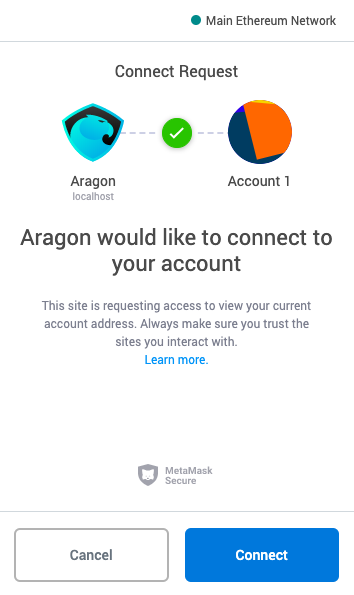
\includegraphics[width=0.4\textwidth]{Figures/metamask.png}
        \caption[Interfaz de metamask]{Interfaz de metamask cuando se pide permiso para conectar a una página. Wiki de Aragon. \cite{web:aragon}}
        \label{fg:aragon}
    \end{figure}
    Después de tener una conexión con su cartera \ref{fg:aragon}, necesitamos una vez mas su permiso. Como hemos comentado en el punto \textit{Introducción a la criptografía}, necesitamos la clave publica de la cartera. Es con esta clave con la que conseguiremos encriptar y desencriptar la información.
    \begin{lstlisting}
        const publicKey = await window.ethereum
			.request({
				method: 'eth_getEncryptionPublicKey',
				params: [account]
			});
    \end{lstlisting}
    De la siguiente forma, llamando al método \verb|eth_getEncryptionPublicKey| la podemos obtener. Nuevamente, para recordar, metamask vive \textit{fuera} de la \textit{burbuja de ejecución} de nuestro dominio. Esto significa que de manera literal necesitamos pedir permiso para realizar cualquier operación con la cartera del usuario.
    \item \textbf{Interactúa con una sala}\\
    \begin{itemize}
        \item \textbf{Crea la sala}\\
        Andes de crear esa sala, se necesitará generar las claves para definir la base de datos como una base de datos privada.
        \begin{lstlisting}
            const identity = await Identities.createIdentity(options);
        \end{lstlisting}
        Cuando ya tenemos nuestra identidad que va a ser usada para el transporte y para los permisos de escritura, podemos empezar a crear la sala.
        Esta sala es una base de datos que como se ha comentado anteriormente será \textbf{keyvalue}.
        \begin{lstlisting}
            const db = await orbitdb.keyvalue(account, options);
            await db.put(account, DID_safe);
        \end{lstlisting}
        Subimos nuestro DID para que el resto de personas puedan verlo al entrar y enviarnos información.
        Por ultimo, solo queda contactar con el smart contract con los métodos anteriormente vistos para poder avisar al resto de usuarios y actualizar la interfaz para avisar al usuario.
        \begin{lstlisting}
            contract.current.methods.createRoom(db.address.toString()).send({ from: account, gasPrice: '20000000000' });
        \end{lstlisting}
        A partir de este momento, otros usuarios pueden haber solicitado entrar en nuestra sala. Gracias a los métodos de escucha se traduce en unas notificaciones en la interfaz del usuario.
        Si decide aceptar alguna de esas notificaciones, se ejecutará las siguientes instrucciones.
        \begin{lstlisting}
            const jsonInterface = JSON.parse(identity);
        \end{lstlisting}
        Leemos la identidad que obtenemos del smart contract y lo parseamos con la clase JSON.
        \begin{lstlisting}
            await DB.current.access.grant('write', jsonInterface.id);
        \end{lstlisting}
        Finalmente podemos añadirle al grupo de personas capaces de escribir en la base de datos.
        \begin{lstlisting}
            contract.current.methods.acceptProposal(proposer).send({ from: account, gasPrice: '20000000000' });
        \end{lstlisting}
        Lógicamente, solo queda avisar al solicitante que puede conectarse.
        \item \textbf{Se una a una sala}\\
        Si el usuario quiere unirse a una sala existente, la secuencia de ejecución es diferente.
        Al igual que si queremos crear una sala, necesitamos generar las claves.
        \begin{lstlisting}
            const identity = await Identities.createIdentity(options);
        \end{lstlisting}
        Al no tener que iniciar la conexión por ahora, simplemente actualizamos la UI para avisar al usuario que toca esperar y solicitamos al smart contract la creación de una petición de entrada.
        \begin{lstlisting}
            contract.current.methods.createProposal(owner, JSON.stringify(identity)).send({ from: account, gasPrice: '20000000000' });
        \end{lstlisting}
        En algún momento, nuestra solicitud será aceptada y podremos conectarnos a la base de datos.
        \begin{lstlisting}
            const db = await orbitdb.open(url, {type: 'keyvalue'});
        \end{lstlisting}
        Abrimos la base de datos especificando la dirección obtenida desde el smart contract.
        \begin{lstlisting}
            // Replicate db in local storage
            await db.load();
        \end{lstlisting}
        Replicamos la base de datos, es decir, pedimos por PUBSUB a cualquier nodo si conoce la información y nos la puede proporcionar.
        \begin{lstlisting}
            await db.put(account, DID_safe);
        \end{lstlisting}
        Y finalmente, podemos subir nuestro nuestro DID para que nos puedan enviar fichero.
    \end{itemize}
    \item \textbf{Interactuamos con los peers}\\
    Como ya hemos compartido toda la información necesaria para hacer nuestro handshake distribuido, es hora de compartir información.
    Gracias a los eventos de replica de orbit db, podemos tener una cuenta de todos los usuarios y sus DID.
    Cuando un usuario quiere enviar un archivo a otro usuario, como se ha especificado en Estado del arte/Criptografía, tenemos que generar una clave común de encriptación/desencriptación y crear una \textit{caja} con esa clave de contenido.
    \begin{lstlisting}
        const syncKey = window.crypto.randomUUID();
        const encryptedSyncKey = encrypt(syncKey, peers[selectedAddress].publicKey);
    \end{lstlisting}
    Después de generar esa caja, solo queda encriptar el fichero y subirlo a IPFS.
    \begin{lstlisting}
        const file = await ipfs.current.add({ content: resultbytes });
        await DB.current.put(
			'to' + selectedAddress + '-' + window.crypto.randomUUID(),
			payload
		);
    \end{lstlisting}
    Para acabar, al ser una base de datos \textbf{keyvalue}, lo marcamos con \verb|tox823...-231324234124|. De esta forma podemos dividir la clave en dos por el guion y leer multiples ficheros sin necesidad de tener colisiones de nombres.
    El usuario que quiera descargar esa información, necesita desencriptar la \textit{caja}.
    \begin{lstlisting}
        const syncKey = await window.ethereum.request({
			method: 'eth_decrypt',
			params: [hexToDecrypt, account],
        });
    \end{lstlisting}
    Tenemos que solicitar permiso al usuario ya que vamos a usar su clave privada. Aunque no podemos verla porque \textbf{nunca} tenemos acceso a su clave privada.
    \begin{lstlisting}
        const stream = ipfs.current.cat(file.path);
    \end{lstlisting}
    Como ya tenemos la clave para abrir el fichero, podemos leer los contenidos y hacer el proceso contrario.
    \begin{lstlisting}
        const blob = new Blob([plaintextbytes], { type: 'application/download' });
        const blobUrl = URL.createObjectURL(blob);
        const FileSaver = require('file-saver');
        FileSaver.saveAs(blobUrl, fileName);
    \end{lstlisting}
    Por ultimo, importamos una librería ara poder descargar el fichero al usuario. 
    Estos pasos son repetibles todas las veces que se quieran y los ficheros están disponibles hasta que algún nodo de la red tenga ese fichero. También se puede \textit{pinnear} el fichero en un nodo remoto. Por ejemplo en los servidores de la universidad de Deusto.
\end{enumerate}
\newpage
\thispagestyle{empty}